\documentclass{multi}

\date{2017 October 2 (Monday)}
\title{Conservative Vector Fields and Introduction to Flux}
\course{Math 60: Multivariable Calculus}

\begin{document}

\emph{Conservative} vector fields are just \emph{gradient} vector fields. To say
that some function \(\vec F\) is a gradient field is to say that there is some
\(f\) such that \(\vec F = \nabla f\).

Notice that the integral of a gradient vector field along a curve \(C\) is thus
the \emph{change} in the potential function across the endpoints of the curve:
\[
    \int_C \vec F \cdot \diff \vec s = \int_C (\nabla f) \cdot \diff \vec s =
    \int_C \left(\frac{\partial f}{\partial x_i} \, \diff x_i + \dots\right) =
    \int_C \diff f = f(\vec b) - f(\vec a),
\]
where \(\vec b, \vec a\) are the endpoints of the curve \(C\).

\paragraph{Example}

Not all vector fields are gradient vector fields! Consider the field \(\vec
F\colon \real^2 \to \real^2 = (-y, x)\), integrated from point \(P\) to point
\(Q\) along two different paths \(C_1\) and \(C_2\):
\begin{center}
  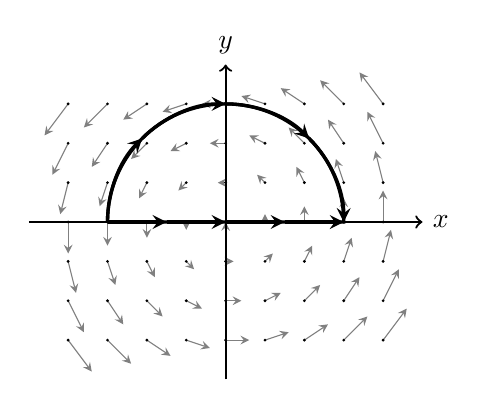
\begin{tikzpicture}[scale=1/2]


\tikzstyle{ax} = [thick, ->]
\tikzstyle{curve} = [very thick, -stealth]

\foreach \i in {-4,...,4} {
  \foreach \j in {-3,...,3} {
  
    \draw[-stealth, gray]
      (\i,\j)
      coordinate[circle, inner sep=.4, fill=black]
      --
      +({-\j/5},{\i/5});
  }
}

\draw[ax]
  (-5,0) -- (5,0)
  node[right]{\(\uvec x\)};

\draw[ax]
  (0,-4) -- (0,4)
  node[above]{\(\uvec y\)};

\draw[very thick]
  (-3,0) -- (3,0)
  arc[radius=3, start angle=0, end angle=180];

\foreach \i in {0,...,3} {
  \draw[curve]
    ({-3+(6/4)*\i},0) -- +({6/4},0);

  \draw[curve]
    ({180-\i*45}:3)
    arc[radius=3, start angle={180-\i*45}, end angle={180-(\i+1)*45}]; 
}
%\draw[curve]
%  (-3,0) -- (0,0);
%
%\draw[curve]
%  (0,0) -- (3,0);
%
%\draw[curve]
%  (3,0) arc[radius=3, start angle=0, end angle=90];
%
%\draw[curve]
%  (0,3) arc[radius=3, start angle=90, end angle=180];
%
%
%



\end{tikzpicture}

\end{center}
Based on the geometry, we notice that the field is perpendicular to the
\(x\)-axis everywhere along the \(x\)-axis, so that the integral

% -y, x plot
% c1 is flat diameter path
% c2 is circular semi above horizontal path
% both left to right
% difference is given by green's theorem
Then consider the curve \(C = C_1 \cup (-C_2)\), so that \(C\) is the boundary
of the semicircular region \(D\). Then by Green's theorem
\[
    \oint_{\partial D = C} \vec F \cdot \diff \vec s = \iint_D
    \left(\frac{\partial N}{\partial x} - \frac{\partial M}{\partial y}\right)
    \diff A,
\]
where \(\vec F(x, y) = (M(x, y), N(x, y))\). Specifically

In general, these two different \emph{path integrals} are not equal. Vector
fields are typically not conservative.

But when are they equal? Notice by Green's theorem that a closed-curve path
integral in a curve like this is zero iff
\[
    \frac{\partial N}{\partial x} - \frac{\partial M}{\partial y}.
\]
Geometrically, notice then that this condition means that the vector field has
no ``rotation'' in the plane.

But also notice that, the reverse implication
\[
    \text{\(\vec F\) is conservative} \impliedby \frac{\partial N}{\partial x} -
    \frac{\partial M}{\partial y} = 0
\]
only holds when \(D\) is ``simply-connected'' (there are no ``holes'' in \(D\)).

\section*{Fundamental Theorem of Line Integrals}

If path \(C\) starts at point \(A\), ends at point \(B\), and \(\vec F = \nabla
f\), then
\[
    \int_C \vec F \cdot \diff \vec s = f(B) - f(A).
\]
Notice that if \(F\) is conservative, the integral over the curve depends
\emph{only} on the endpoints, not on the path taken!

\paragraph{Example}

Consider the vector field \(\vec F = (2x, 2y)\). Calculate the path integral
over \(C\), a straight line from \((1, 1)\) to \((4, 3)\).

We can compute the integral by parametrizing the curve and integrating over the
parametrized curve.

We can also compute the integral by evaluating the potential function \(f = x^2
+ y^2\).

\section*{Flux}

The flux is a double integral of a vector field over a surface:
\[
    \iint_S \vec F \cdot \diff \vec S
\]
where \(\diff \vec S\) is some sort of a differential \emph{area} vector (a
vector normal to the surface with differential area \(|\diff \vec S|\)).
\begin{center}
  \input{flux.tikz}
\end{center}

% visualizations???
% curved surface with vector field flying around
% highlight a small square 
% flat surface, vector field going straight up or slanted to the side
% see projections


\end{document}
